\section{Descrizione dello schema per la persistenza dati}
La gestione della persistenza dei dati è centrale per il nostro backend e si basa su un modello che sfrutta le potenzialità di Hibernate.  PostgreSQL, per la loro affidabilità e diffusione nell’ecosistema Java.

Hibernate si occupa di:

Mappare le entità: Le classi Java rappresentano le entità del dominio, le quali vengono automaticamente correlate alle tabelle del database.
Gestire le relazioni: Le associazioni fra le entità (uno-a-uno, uno-a-molti, molti-a-molti) sono gestite in modo trasparente, riducendo la complessità nella scrittura delle query.
Ottimizzare le operazioni di lettura e scrittura: Grazie al supporto per caching e gestione delle transazioni, Hibernate semplifica l’interazione con il DBMS e contribuisce a mantenere il sistema performante e affidabile.
\newpage
\begin{figure}
	\centering
	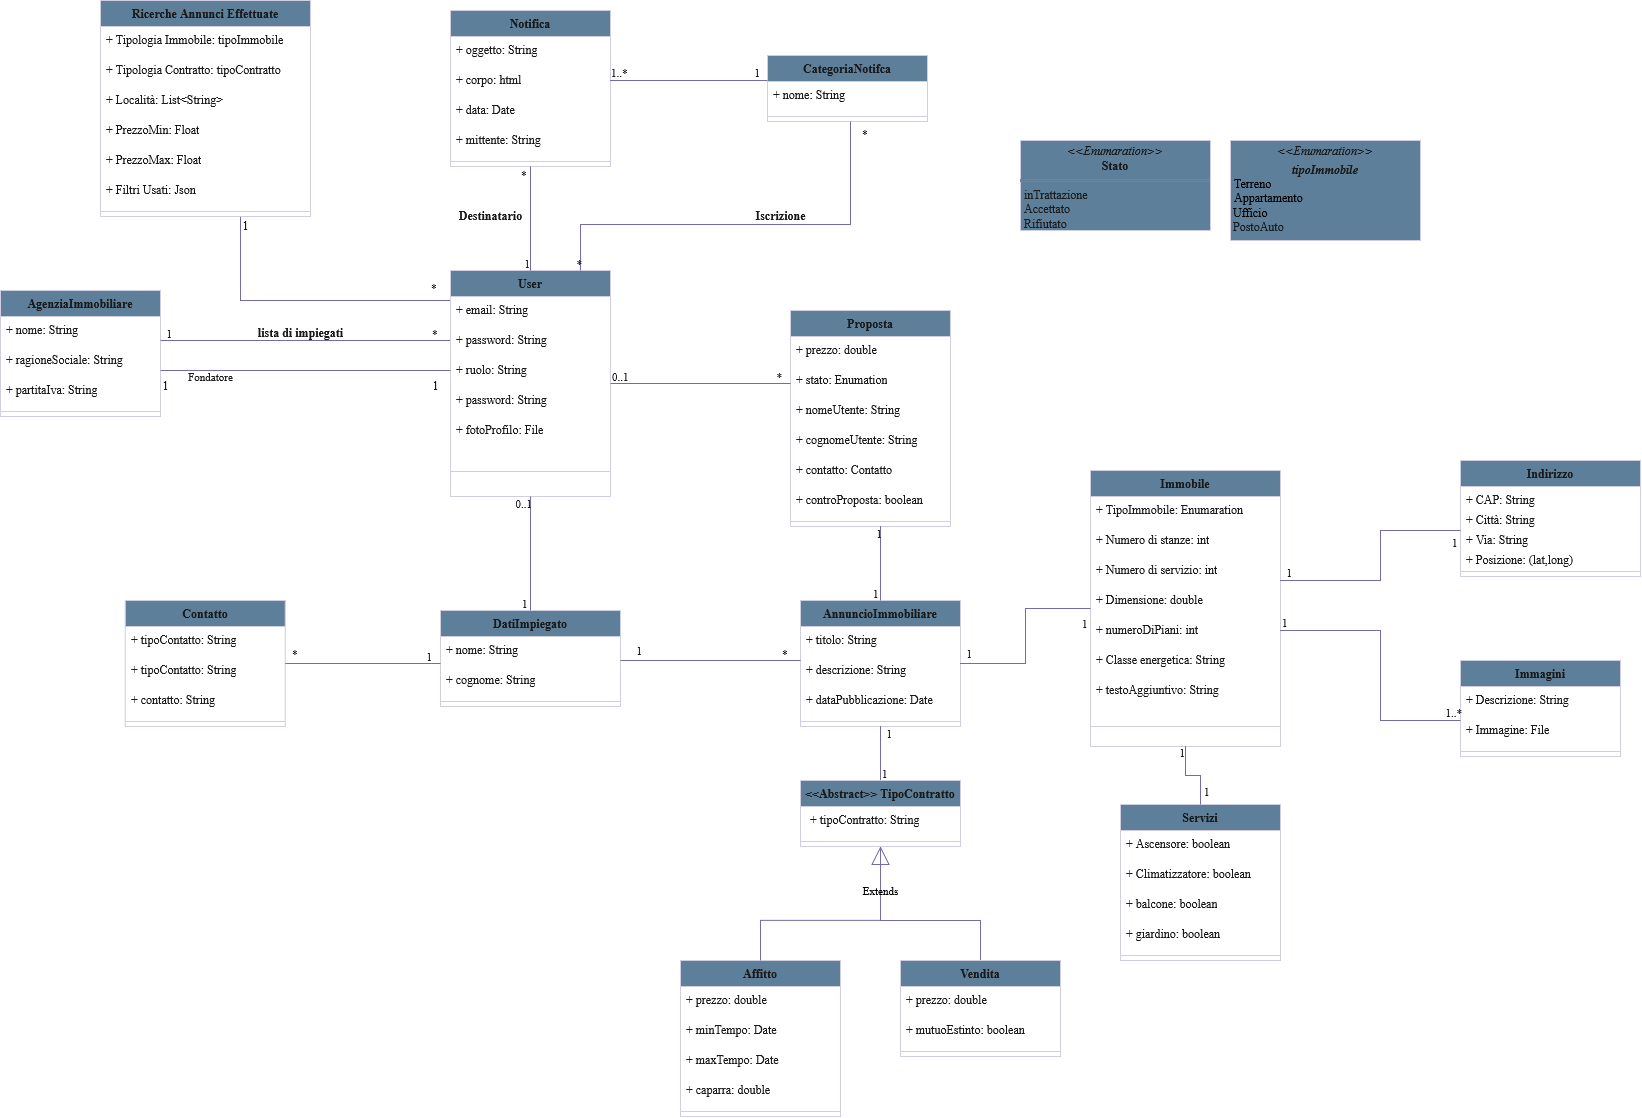
\includegraphics[width=1
	\linewidth]{Immagini/diagramma delle classi.drawio.png}
	\caption{Diagramma delle classi usate}
	\label{fig:enter-label}
\end{figure}
